\chapter{Installation}

\section{MS-Windows}


To install InVesalius on MS-Windows, simply run the installer program. When a window asking you to confirm the file execution appears, click \textbf{Yes}.

\begin{figure}[!htb]
\centering
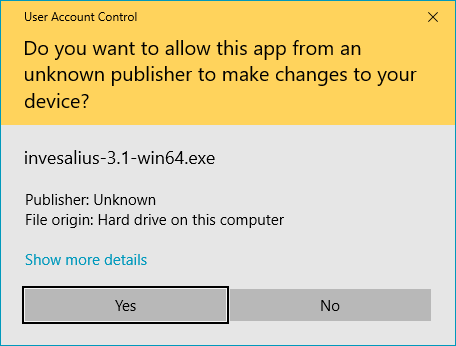
\includegraphics[scale=0.5]{installation_exec_en.png}
\end{figure}

\newpage

A new window will ask you to select the language of the installer. Select the language and click \textbf{OK} button.

\begin{figure}[!htb]
\centering
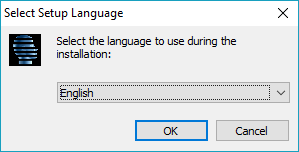
\includegraphics[scale=0.7]{installation_select_language_en.png}
\end{figure}
 
\hspace{.2cm}

Window installer appears. Click \textbf{Next}.


\begin{figure}[!htb]
\centering
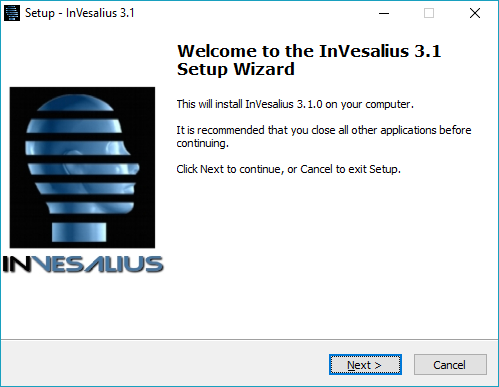
\includegraphics[scale=0.7]{installation_welcome_en.png}
\end{figure}

\newpage

Select \textbf{I accept the agreement} and click on \textbf{Next} button.

\begin{figure}[!htb] 
\centering
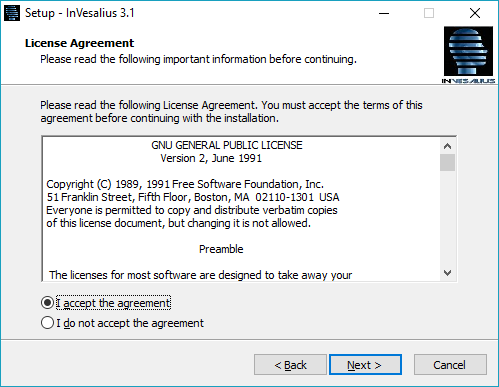
\includegraphics[scale=0.7]{installation_license_en.png}
\end{figure}

\hspace{.2cm}

Click on \textbf{Next} button again. 

\begin{figure}[!htb]  
\centering
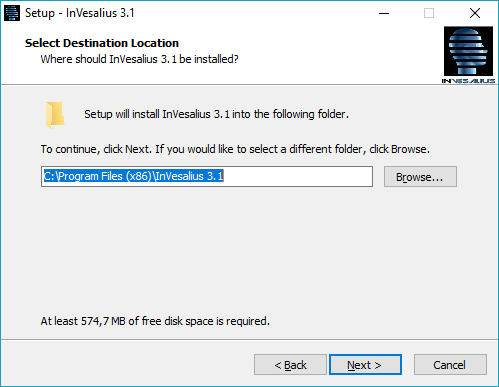
\includegraphics[scale=0.7]{installation_folder_en.png}
\end{figure}

\newpage

Click on \textbf{Next}  button.
\begin{figure}[!htb]
\centering
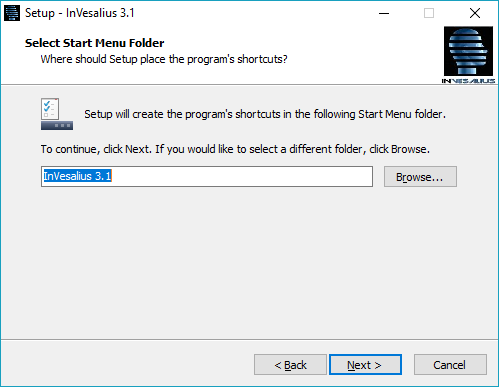
\includegraphics[scale=0.7]{installation_program_name_en.png}
\end{figure}

\hspace{.2cm}

Select \textbf{Create a desktop shortchut} and click on \textbf{Next}.

\begin{figure}[!htb]
\centering
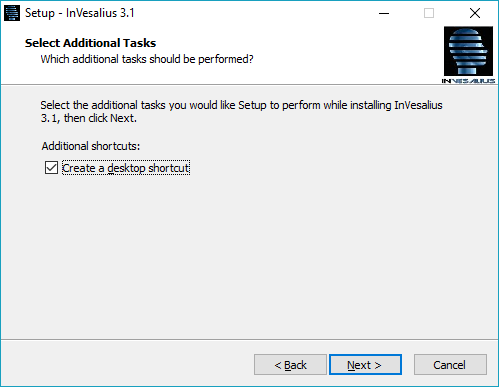
\includegraphics[scale=0.7]{installation_desktop_shortcut_en.png}
\end{figure}

\newpage

Click on \textbf{Install} button.

\begin{figure}[!htb]
\centering
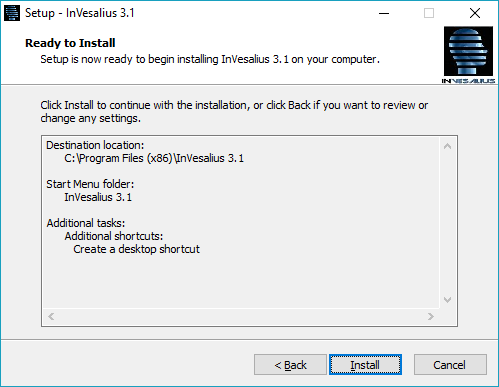
\includegraphics[scale=0.7]{installation_resume_en.png}
\end{figure}

\hspace{.2cm}

While the software is installed, a progress window will appear.

\begin{figure}[!htb]
\centering
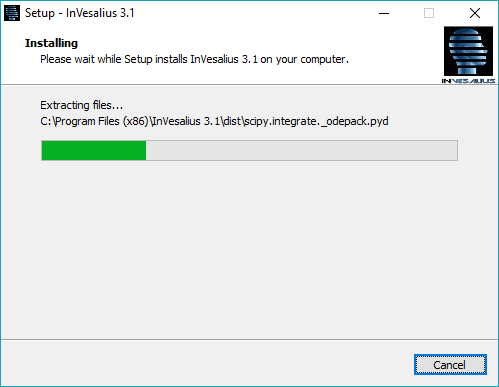
\includegraphics[scale=0.7]{installation_progress_en.png}
\end{figure}

\newpage

To run InVesalius after installation, check \textbf{Lauch InVesalius 3.1} and click on \textbf{Finish} button.

\begin{figure}[!htb]
\centering
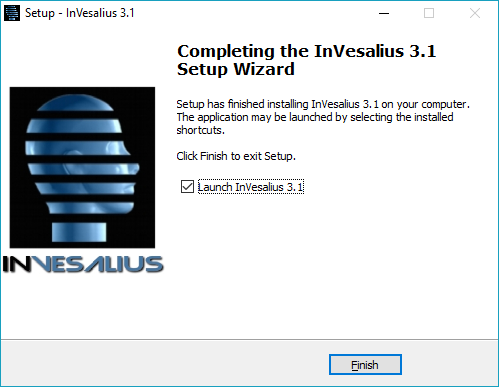
\includegraphics[scale=0.7]{installation_finish_en.png}
\end{figure}

\hspace{.2cm}

If this is the first time the software is installed, a window will appear to select the InVesalius language. Select the language you want and click on \textbf{OK} button.

\begin{figure}[!htb]
\centering
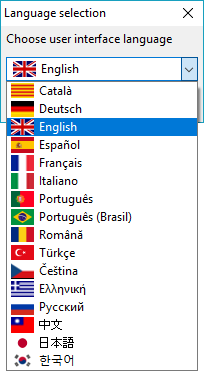
\includegraphics[scale=0.6]{invesalius_language_select_en.png}
\end{figure}

\newpage

While InVesalius is loaded, an opening window like the one in the next figure is displayed.

\begin{figure}[!htb]
\centering
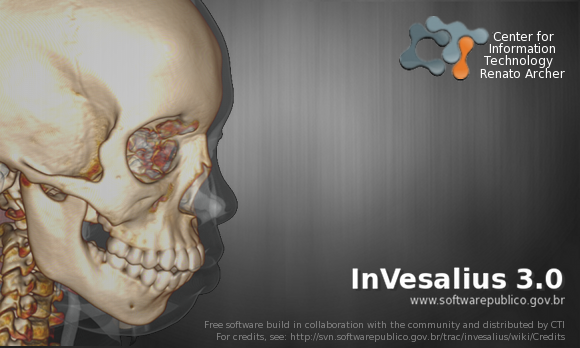
\includegraphics[scale=0.4]{splash_en.png}
\end{figure}

\hspace{.2cm}

Then, the main program window open.

\begin{figure}[!htb]
\centering
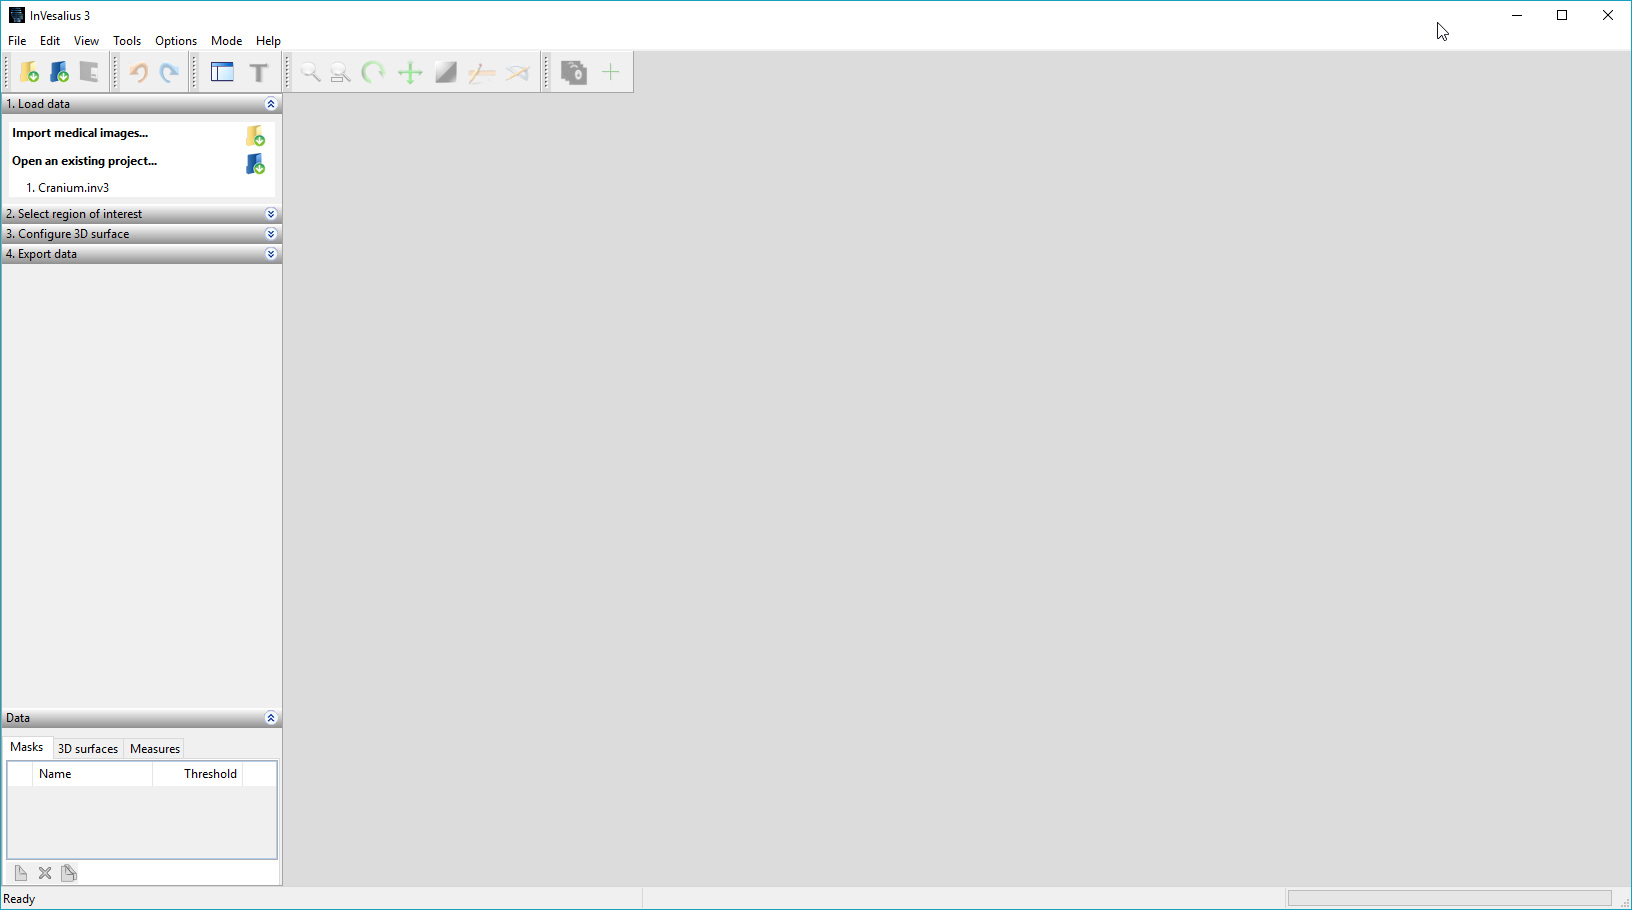
\includegraphics[scale=0.3]{main_window_without_project_en.png}
\end{figure}

\section{Mac Os X}

To start the installation on Mac Os X, double-click the installer with the left mouse button.
Then the installer will be initialized.

\begin{figure}[!htb]
\centering
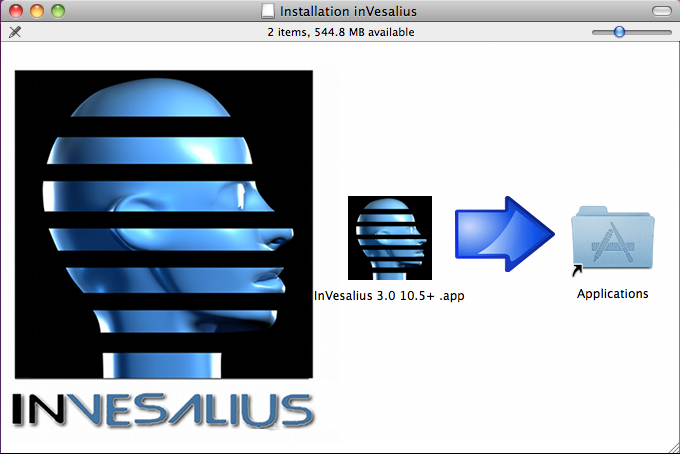
\includegraphics[scale=0.3]{mac2.png}
\end{figure}

Hold down the left button on the InVesalius software icon and drag it to the \textit{Applications}. Both contained in the installer.

\begin{figure}[!htb]
\centering
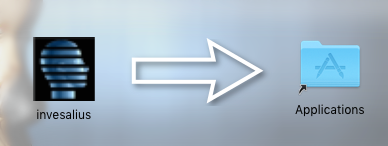
\includegraphics[scale=0.4]{mac4.png}
\end{figure}

The software is already installed, just access through the menu.